\documentclass[10pt,twoside]{fernandes_supp} 
%Default opts:9pt,twocolumn,twoside
\graphicspath{{images_supp/}}

\newcommand{\KB}[1]{\noindent\color{blue}$\Longrightarrow$ #1\normalcolor}
\newcommand{\mf}[1]{\colorbox{blue!10}{\color{color3}#1}}

\title{Supplemental Information:\\ Harnessing  Design Principles from Glass Sponges for Structurally Robust Lattice Structures}

\author[1]{Matheus C. Fernandes}
\author[2]{James C. Weaver}
\author[1,3,*]{Katia Bertoldi}

\affil[1]{John A. Paulson School of Engineering and Applied Sciences -- Harvard University, Cambridge, MA 02138}
\affil[2]{Wyss Institute -- Harvard University, Cambridge, MA 02138}
\affil[3]{Kavli Institute -- Harvard University, Cambridge, MA 02138}
\affil[*]{Corresponding author: \href{mailto:bertoldi@seas.harvard.edu}{bertoldi@seas.harvard.edu}}

\begin{document}
\maketitle
% \doublespace
% \linenumbers
\section{Structure of the Hexactinellid sponge \textit{Euplectella aspergillum}}\label{sec:params}
The periodic structures investigated in this study are inspired by the skeleton of the Hexactinellid sponge \textit{Euplectella aspergillum (sp.)}, commonly known as the "Venus' flower basket". In this section we provide a detailed description of the sponge geometry and measured dimensions.

\Cref{Sponge} shows a photograph of the entire skeleton of the \textit{Euplectella sp.}, and its intricate, cylindrical cage-like structure (20 to 25cm long, 2 to 4 cm in diameter) \citep{aizenberg2005}. The surface of the cylinder consists of a regular square lattice composed of a series of cemented vertical and horizontal struts with circular cross-section. The cell spacing between horizontal and vertical struts was reported  to be $L\approx 2.5$mm \citep{weaver2007}, while their diameter was measured to be $D_{nd}\approx 0.25$mm \citep{weaver2007}. Besides the horizontal and vertical struts, there is an additional set of diagonal elements, intersecting in a manner that creates a series of alternating open and closed cells, reminiscent of a checkerboard pattern \citep{weaver2007}. Although these diagonal elements are not as ordered as the horizontal and vertical ones, it has been shown that they can be approximated with two diagonal struts that are offset from the nodes  (vertex joints between non-diagonal elements) and form octagonal openings (\cref{Sponge}(d)). To estimate the volume ratio between diagonal and non-diagonal elements, we took high resolution photographs of the sponge and performed image segmentation to segregate the projected area of the vertical/horizontal and diagonal spicules. Using this approach, the projected area ratio of non-diagonal to diagonal elements was found to be $A_{nd}/A_{d}\approx1.4$. Note that here, and in the following, the subscripts $d$ and $nd$ are used to indicate diagonal and non-diagonal (i.e. horizontal and vertical) elements, respectively. 

Finally, it should also be noted that the sponge is reinforced by external ridges that extend perpendicular to the surface of the cylinder and spiral the cage at an angle of $45^\text{o}$. However, in this paper we do not report the effects of these ridges on it's structural performance.

\begin{figure}[H]
    \centering
    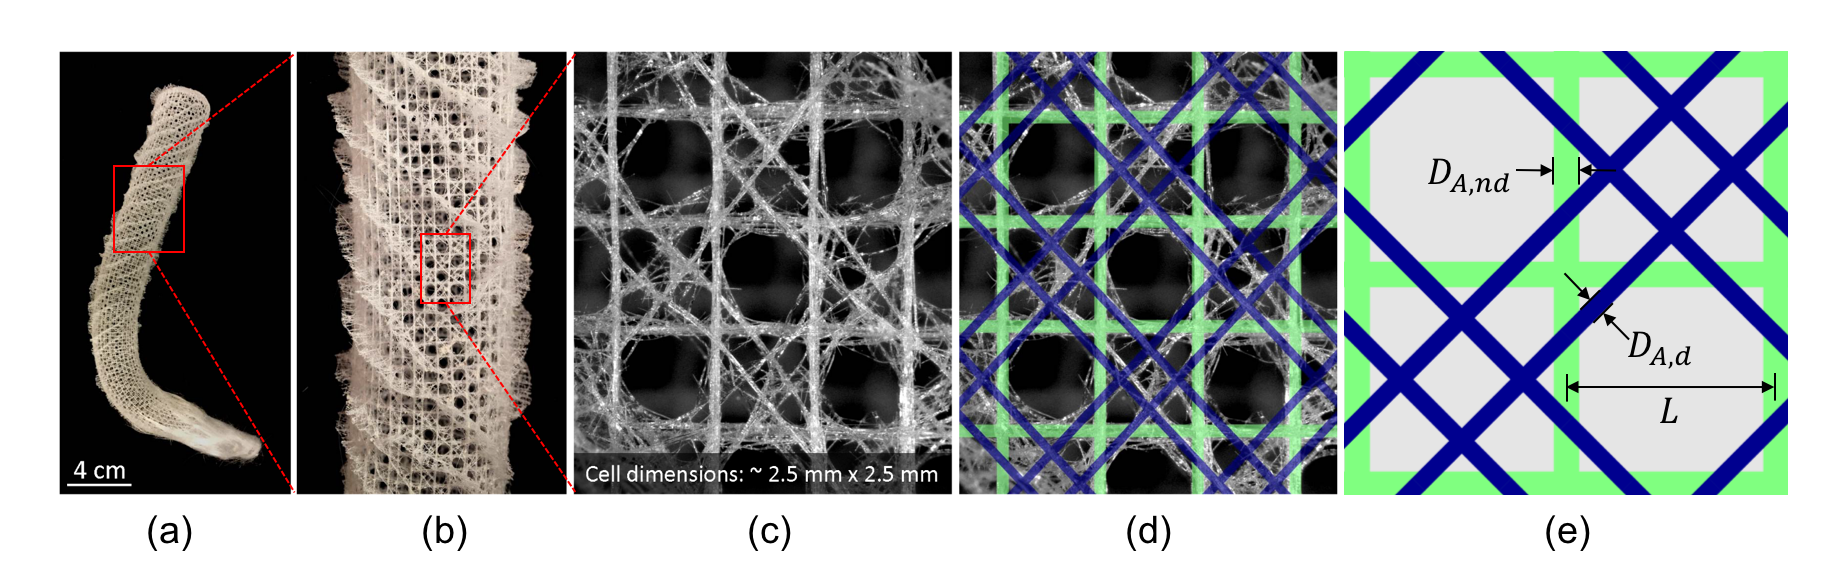
\includegraphics[width=0.9\linewidth]{SFig1.png}
    \caption{\textbf{Hexactinellid sponge \textit{Euplectella aspergillum.}} (a)-(b) Full-frame photo of sponge.  (c)  Close up microscope image of the sponge. (d) Comparison between the idealized model (green and blue lines) and the sponge structure. (e) Unit cell of the idealized model.}
    \label{Sponge}
\end{figure}

\section{Designs Considered}\label{sec:designs}
In this study, we focus on four different lattice configurations constrained to deform in an in-plane setting only. In an effort to conduct a fair performance comparison between the different designs, the total volume of material is conserved. Moreover,  we consider a fixed volume ratio between non-diagonal and diagonal elements (chosen to match the sponge geometry) as well as two different shapes for the cross section of all lattice members: circular and rectangular.  For the circular cross-section case  we stay consistent with the geometry found within the biological species. However, since slender members with such circular cross-section easily buckle out-of-plane when subject to compression loading, we also consider  rectangular cross-sections and choose the depth to slenderness ratio  sufficiently large to avoid out-of-plane deformation. 

In the subsequent sections, we describe in detail the unit cells for four different designs (Designs A-D), and provide the derivations for each geometry cross-section characteristics. 

\subsection{Design A}
Design A is inspired by the sponge structure and consists of a square grid  reinforced by a double diagonal system (see \cref{DesignA}). 
\subsubsection{Circular cross section} 
If we assume that the horizontal and vertical struts have length $L$ and circular cross section  with diameters $D_{A,nd}$, their volume and projected-area in the unit cell are given by 
\begin{equation}\label{V1}
V_{A,nd}=8 L \left(\pi\frac{D^2_{A,nd}}{4}\right)=2 L \pi D^2_{A,nd}
\end{equation}
and
\begin{equation}\label{A1}
A_{A,nd}=8 L D_{A,nd},
\end{equation}
respectively. Note that in this study we use 
\begin{equation}
\frac{D_{A,nd}}{L}=0.1,
\end{equation}
since this is the aspect ratio measured for the sponges (see \cref{sec:params}).

Moreover, as for the case of the sponge, the diagonal elements are assumed to form an octagonal opening on every other cell. As such, the diagonals intersect the horizontal and vertical struts at a distance $\Delta L=L/(\sqrt{2}+2)$ from the nodes and their  volume and projected area in the unit cell are
\begin{equation}\label{V2}
V_{A,d}=8 \sqrt{2} L\left(\pi\frac{D^2_{A,d}}{4}\right)=2\sqrt{2}L \pi D^2_{A,d},
\end{equation}
and
\begin{equation}\label{A2}
A_{A,d}=8\sqrt{2} L D_{A,d},
\end{equation}
respectively. Since the projected area ratio of the non-diagonal to diagonal elements in the sponge has been measured to be 
\begin{equation}
\frac{A_{A,nd}}{A_{A,d}}=1.4,
\end{equation}
by substituting \cref{A1} and \cref{A2} into the equation above we find that for Design A
\begin{equation} \label{DA}
D_{A,nd}=1.4\sqrt{2}D_{A,d}\approx 2 D_{A,d}.
\end{equation}
Substitution of \cref{DA} into \cref{V1} and \cref{V2} yields 
\begin{equation}
\frac{V_{A,nd}}{V_{A,d}}=\frac{2 L \pi D^2_{A,nd}}{2\sqrt{2}L \pi D^2_{A,d}}=2\sqrt{2}
\end{equation}
and
\begin{equation}\label{VT}
V_{A,T}=V_{A,nd}+V_{A,d}=2\pi L (D_{A,nd}^2+\sqrt{2} D_{A,d}^2)=2\pi L D_{A,nd}^2 \left(1+\frac{1}{2\sqrt{2}}\right),
\end{equation}
where $V_{A,T}$ indicates the total volume of the unit cell for Design A. 

Finally, it is important to note that in this study we use Design A as our base model, and thus constrain the total volume of all the other unit cell designs to be equal to that of Design A, namely,
\begin{equation}\label{con1}
V_{\alpha,d}+V_{\alpha,nd}={V}_{A,T}=2\pi L D_{A,nd}^2 \left(1+\frac{1}{2\sqrt{2}}\right),
\end{equation}
with $\alpha=$ B, C and D.
For Designs B and C, which comprise diagonal elements, we also  constrain the volume ratio of the non-diagonal to diagonal elements to be the same as in Design A
\begin{equation}\label{con2}
\frac{V_{\alpha,nd}}{V_{\alpha,d}}=\frac{V_{A,nd}}{V_{A,d}}=2\sqrt{2},
\end{equation}
with $\alpha=$ B and C.

\begin{figure}[H]
    \centering
    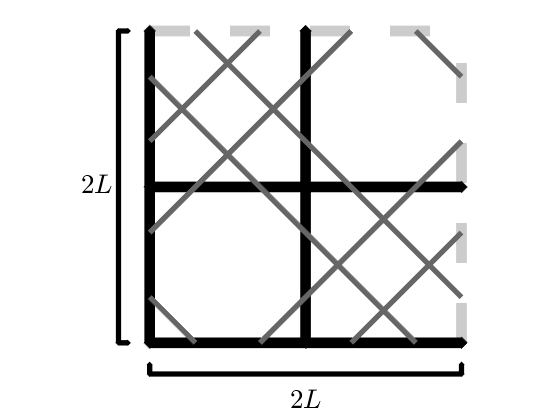
\includegraphics[width=0.4\linewidth]{SFig2.png}
    \caption{{\bf Unit cell for Design A.} This design is inspired by the sponge structure and consists of a square grid  reinforced by a double diagonal system. The horizontal and vertical struts have length $L$ and circular cross section with diameter $D_{A,nd}$ and, as with the sponge, we assume $D_{A,nd}/L=0.1$. The diagonal elements have a circular cross section  with diameter $D_{A,d}=2 D_{A,nd}$.}
    \label{DesignA}
\end{figure}

\subsubsection{Rectangular cross-section}

Based on biological observations we can infer the ratio of non-diagonal to diagonal strut cross-sectional area to be  $A_{nd}/A_d\approx 1.4$. Using this information, we can develop the total volume ratio of non-diagonal to diagonal members to be $V_{nd}/V_d\approx 1.4$ assuming a uniform in-plane thickness $h$ for all struts. Using our sponge geometry interpretation we can obtain the following two expressions relating the members volume and thickness $T$:
\begin{equation}
	V_{A,nd}=8LT_{A,nd}h
\end{equation}
\begin{equation}
	V_{A,d}=8\sqrt{2}LT_{A,d}h
\end{equation}
where $V_{A,nd}$, $T_{A,nd}$,$V_{A,d}$ and $T_{A,d}$ are the non-diagonal volume, strut thickness and diagonal volume and strut thickness for Design A, respectively. Let us enter this relationship into our biological observation, which yields:
\begin{equation}
	\frac{V_{A,nd}}{V_{A,d}}\approx 1.4\approx\sqrt{2}=\frac{8LT_{A,nd}h}{8\sqrt{2}LT_{A,d}h}
\end{equation}
Therefore, we can simplify this relationship as
\begin{equation}
	T_{A,nd}=2T_{A,d}
\end{equation}

\subsection{Design B}
Design B is similar to the sponge design (Design A) and is likewise characterized by an alternation of open and closed cells (\cref{DesignB}). However, instead of having two diagonals offset from the nodes, here we only have one diagonal passing through the nodes and crossing every other cell. 

\subsubsection{Circular cross section}
For this design with circular cross section the non-diagonal and diagonal volumes are given by
\begin{equation}
V_{B,nd}=V_{A,nd}=2\pi L D_{B,nd}^2
\end{equation}
and
\begin{equation}
V_{B,d}=2\sqrt{8} L \left(\pi \frac{{D}_{B,d}^2}{4}\right),
\end{equation}
respectively.
Using the constraints provided by \cref{con1} and \cref{con2}, as well as the above volumes, we  obtain 
\begin{equation}
{{D}_{B,nd}}={{D}_{A,nd}}
\end{equation}
and
\begin{equation}
\frac{{D}_{B,d}}{{D}_{B,nd}}=\frac{1}{\sqrt{2}}.
\end{equation}

\begin{figure}[H]
    \centering
    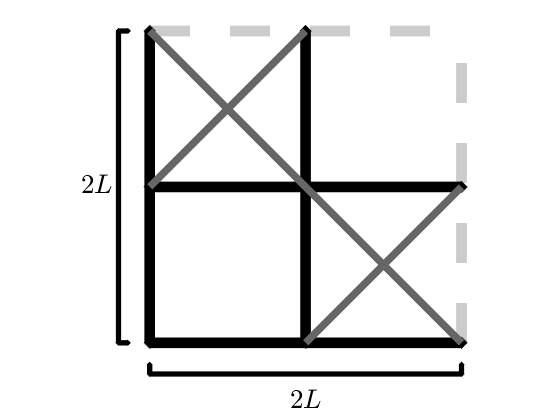
\includegraphics[width=0.4\linewidth]{SFig3.png}
    \caption{{\bf Unit cell for Design B.} This design is still characterized by an alternation of open and closed cells. However, instead of having two  diagonals offset from the nodes, here we only have one diagonal passing through the nodes and crossing every other cell. The horizontal and vertical struts have length $L$ and a circular cross section with diameter $D_{B,nd}$. The diagonal elements have a circular cross section  with diameter $D_{B,d}={D_{B,nd}}/{\sqrt{2}}$.}
    \label{DesignB}
\end{figure}

\subsubsection{Rectangular cross section}
For this design the volume of non-diagonal elements remain the same, namely,
\begin{equation}
		V_{B,nd}=8LT_{B,nd}h.
\end{equation}
However, the volume for the diagonal elements will is different as a result the change in total length, namely,
\begin{equation}
		V_{B,d}=4\sqrt{2}LT_{A,d}h.
\end{equation}
In in effort to maintain a constant volume ration between the diagonally reinforced designs, we use the same volume ratio as per observation
\begin{equation}
		\frac{V_{B,nd}}{V_{B,d}}\approx 1.4\approx\sqrt{2}=\frac{8LT_{B,nd}h}{4\sqrt{2}LT_{B,d}h}
\end{equation}
which simplifies to
\begin{equation}
	T_{B,nd}=T_{B,d}
\end{equation}
and
\begin{equation}
	T_{B,nd}=T_{A,nd}
\end{equation}

\subsection{Design C}
Design C is inspired by the town lattice truss design introduced by architect Ithiel Town in 1820 \citep{waddell1916} and consists of every cell being reinforced by diagonal trusses passing through the nodes (see \cref{DesignC}).

\subsubsection{Circular cross section}
For this design with circular cross section, the non-diagonal and diagonal volumes of the unit cell are given by:
\begin{equation}
V_{C,nd}=V_{A,nd}=2 L \pi D^2_{A,nd}
\end{equation}
and
\begin{equation}
V_{C,d}=V_{A,d}=2\sqrt{2}L \pi D^2_{A,d},
\end{equation}
respectively.
Using the constraints provided by \cref{con1} and \cref{con2} we  obtain 
\begin{equation}
{{D}_{C,nd}}={{D}_{A,nd}}
\end{equation}
and
\begin{equation}
\frac{{D}_{C,d}}{{D}_{C,nd}}=\frac{1}{2}.
\end{equation}

\begin{figure}[H]
    \centering
    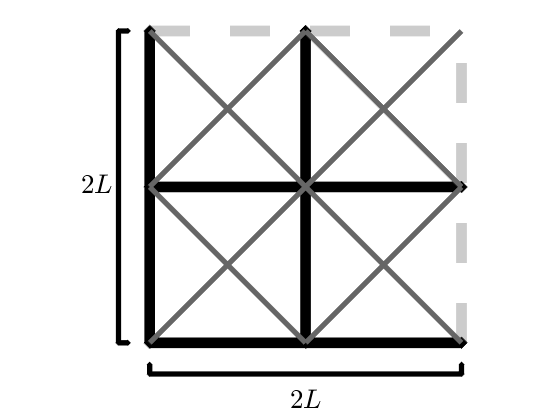
\includegraphics[width=0.4\linewidth]{SFig4.png}
    \caption{{\bf Unit cell for Design C.} This design consists of a square grid with all cells being reinforced by diagonal trusses passing through the nodes.  The horizontal and vertical struts have length $L$ and a circular cross section with diameter $D_{C,nd}$. The diagonal elements have a circular cross section  with diameter $D_{C,d}={D_{C,nd}}/{2}$.}
    \label{DesignC}
\end{figure}

\subsubsection{Rectangular cross section}
Because the total length of the diagonal and non-diagonal elements are the same as for Design A, we obtain the same diameters for the elements, namely,
\begin{equation}
T_{A,nd}=2T_{A,d}
\end{equation}
and
\begin{equation}
T_{C,nd}=T_{A,nd}
\end{equation}

\subsection{Design D} 
Design D comprises only the square grid without diagonal reinforcement (\cref{DesignD}) and is well known to be unstable and very limited in resisting shear forces \citep{gibson1999,deshpande2001}. As such, for this design we allocate the total material volume to the non-diagonal elements.

\subsubsection{Circular cross section}
Since
\begin{equation}
V_{D,T}=V_{D,nd}=V_{A,nd}=2\pi L D_{D,nd}^2,
\end{equation}
using the constraint provided by \cref{con1} we obtain
\begin{equation}
{D_{D,nd}}={D_{A,nd}}\sqrt{1+\frac{\sqrt{2}}{4}}. 
\end{equation}

\begin{figure}[H]
    \centering
    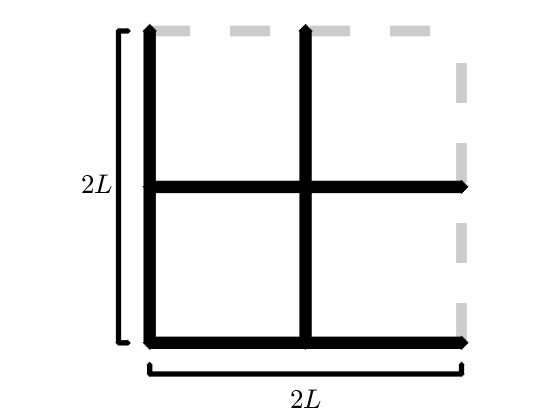
\includegraphics[width=0.4\linewidth]{SFig5.png}
    \caption{{\bf Unit cell for Design D.} This design consists of a square grid without diagonal reinforcement.  The horizontal and vertical struts have length $L$ and a circular cross section with diameter $D_{D,nd}$.}
    \label{DesignD}
\end{figure}

\subsubsection{Rectangular cross-section}
For this design, because it does not contain any diagonal elements, we must allocate the total volume of the structure fully on the non-diagonal elements. Thus we can formulate the total volume of Design A as
\begin{equation}
	V_{A,nd}+V_{A,d}=(T_{A,nd}+\sqrt{2}T_{A,d})8Lh
\end{equation}
Using the relationship between the non-diagonal thickness and diagonal thickness, we obtain
\begin{equation}
V_{A,nd}+V_{A,d}=\left(1+\frac{1}{\sqrt{2}}\right)8LhT_{A,nd}
\end{equation}

We can build a relationship between Design A and Design D through the total volume, such that the total volume of Design A is the same as the total volume of Design D
\begin{equation}
\left(1+\frac{1}{\sqrt{2}}\right)8LhT_{A,nd}=8LhT_{D,nd}
\end{equation}
which yields a relationship between the thicknesses of the non diagonal elements as
\begin{equation}
	T_{D,nd}=\left(1+\frac{1}{\sqrt{2}}\right)T_{A,nd}
\end{equation}

\section{Numerical Model}
The finite element analysis presented in this article were conducted using the {\it ABAQUS/Standard}. All models were constructed using 1D Timoshenko beam  (ABAQUS element type B22) and all beam crossings were assumed to be welded joints. For each instance, seeding of the mesh was chosen to be at least 1/10 of the minimum beam length. The response of the material was captured using a linear elastic model with  Poisson's ratio $\nu=0.3$ and  Young's modulus of $E$.


To reduce the computational cost, we took advantage of the periodicity of the structures and investigated their response  using  a Representative Volume Element (RVE) as seen in \cref{RVE}.
To subject the RVE to a macroscopic deformation gradient $\overline{\mathbf{F}}$ periodic boundary conditions are imposed on all cell boundaries  \citep{danielsson2002, bertoldi2008}
\begin{equation} \label{EQN:DefInfPeriodicFEM}
    u_\alpha^{A_i} -u_\alpha^{B_i} = (\overline{F}_{\alpha\beta}-\delta_{\alpha\beta})(X_\beta^{A_i}-X_\beta^{B_i}), \quad i=1,\,2,\,....,\,N
\end{equation}
where $\delta_{\alpha\beta}$ is the Kronecker delta, $u_\alpha^{A_i}$  and $u_\alpha^{B_i}$ ($\alpha=1,\,2$) are displacements of points periodically located on the boundary of the unit cell. Moreover, $N$ denotes the number of pairs of nodes periodically located on the boundary of the unit cell. For the square lattice considered in this study $N=2$ when the unit cell is considered, while $N=4$ and $N=6$ for the enlarged $2\times2$ and $1\times5$ unit cells, respectively. Note that  the components of $\overline{\mathbf{F}}$ can be conveniently prescribed within the finite element framework using a set of virtual nodes. The corresponding  macroscopic first Piola-Kirchhoff stress $\overline{\mathbf{P}}$ is then obtained through virtual work considerations \citep{danielsson2002, bertoldi2008}. 

In this study the following macroscopic loading condition was considered: 
\KB{add $\overline{\mathbf{F}}$ that you use in the analysis? this should be the most general case. How o you deal with the loading orientation $\theta$? }




 To determine the initial stiffness of the structures  we performed a linear elastic analysis. \KB{ Which one to calculate the stiffness? Explain how do you conduct the analysis with different loading orientations}


For all buckling analysis, we performed a linear stability buckling analysis \KB{did you use *buckling or *frequency? Did you account for the effect of pre-deformation}
\KB{Since buckling may alter the periodicity of the
structure, we considered super cells consisting of $m \times n$
undeformed RVEs subjected to periodic boundary
conditions and calculated the critical strain for each of
them. The critical strain of the infinite periodic structure is
then defined as the minimum critical strain on all considered
super cells. \KB{it would be good to add this plot for each Design. Similar to Fig. 2c in "Complex Ordered Patterns in Mechanical Instability Induced Geometrically
Frustrated Triangular Cellular Structures"}}

\KB{how do you account for different $\theta$?}

\KB{comment on the results}


%For infinite structures modeled using period boundary conditions, it is important to realize the distinction between local instabilities (i.e. instabilities with wavelength that are of the order of the size of the unit cell) and global instabilities (i.e. instabilities with large wavelengths in comparison to the size of the unit cell). In order to capture any global instabilities potentially missed by using the minimum RVE, we further develop our period numerical studies to include RVEs that tessellate the unit cells presented in \cref{sec:designs}. For all designs, we increase the domain size by tessellating up to 20x20 unit cells (creating a base grid of 40x40 square cells). For Designs A-C, the critical bucking strain and modes do not change for larger unit cells suggesting that there does not exist a global instability. Whereas, for Design D, as we increase the domain size (add more unit cells to the tessellation), the instability  wavelength continues to grow with the size of the domain, suggesting a global macroscopic instability that depends on the size of the domain. The critical buckling strain is inversely proportional with the RVE size and approaches 0 in the limit that the RVE size approaches infinity. It is well known and documented that Design D is unstable when loaded in uniaxial compression. 

%\mf{Write about minimum RVE -- how do I convey this message? Should I produce a plot or just verbally state this check?}



\begin{figure}[H]
    \centering
	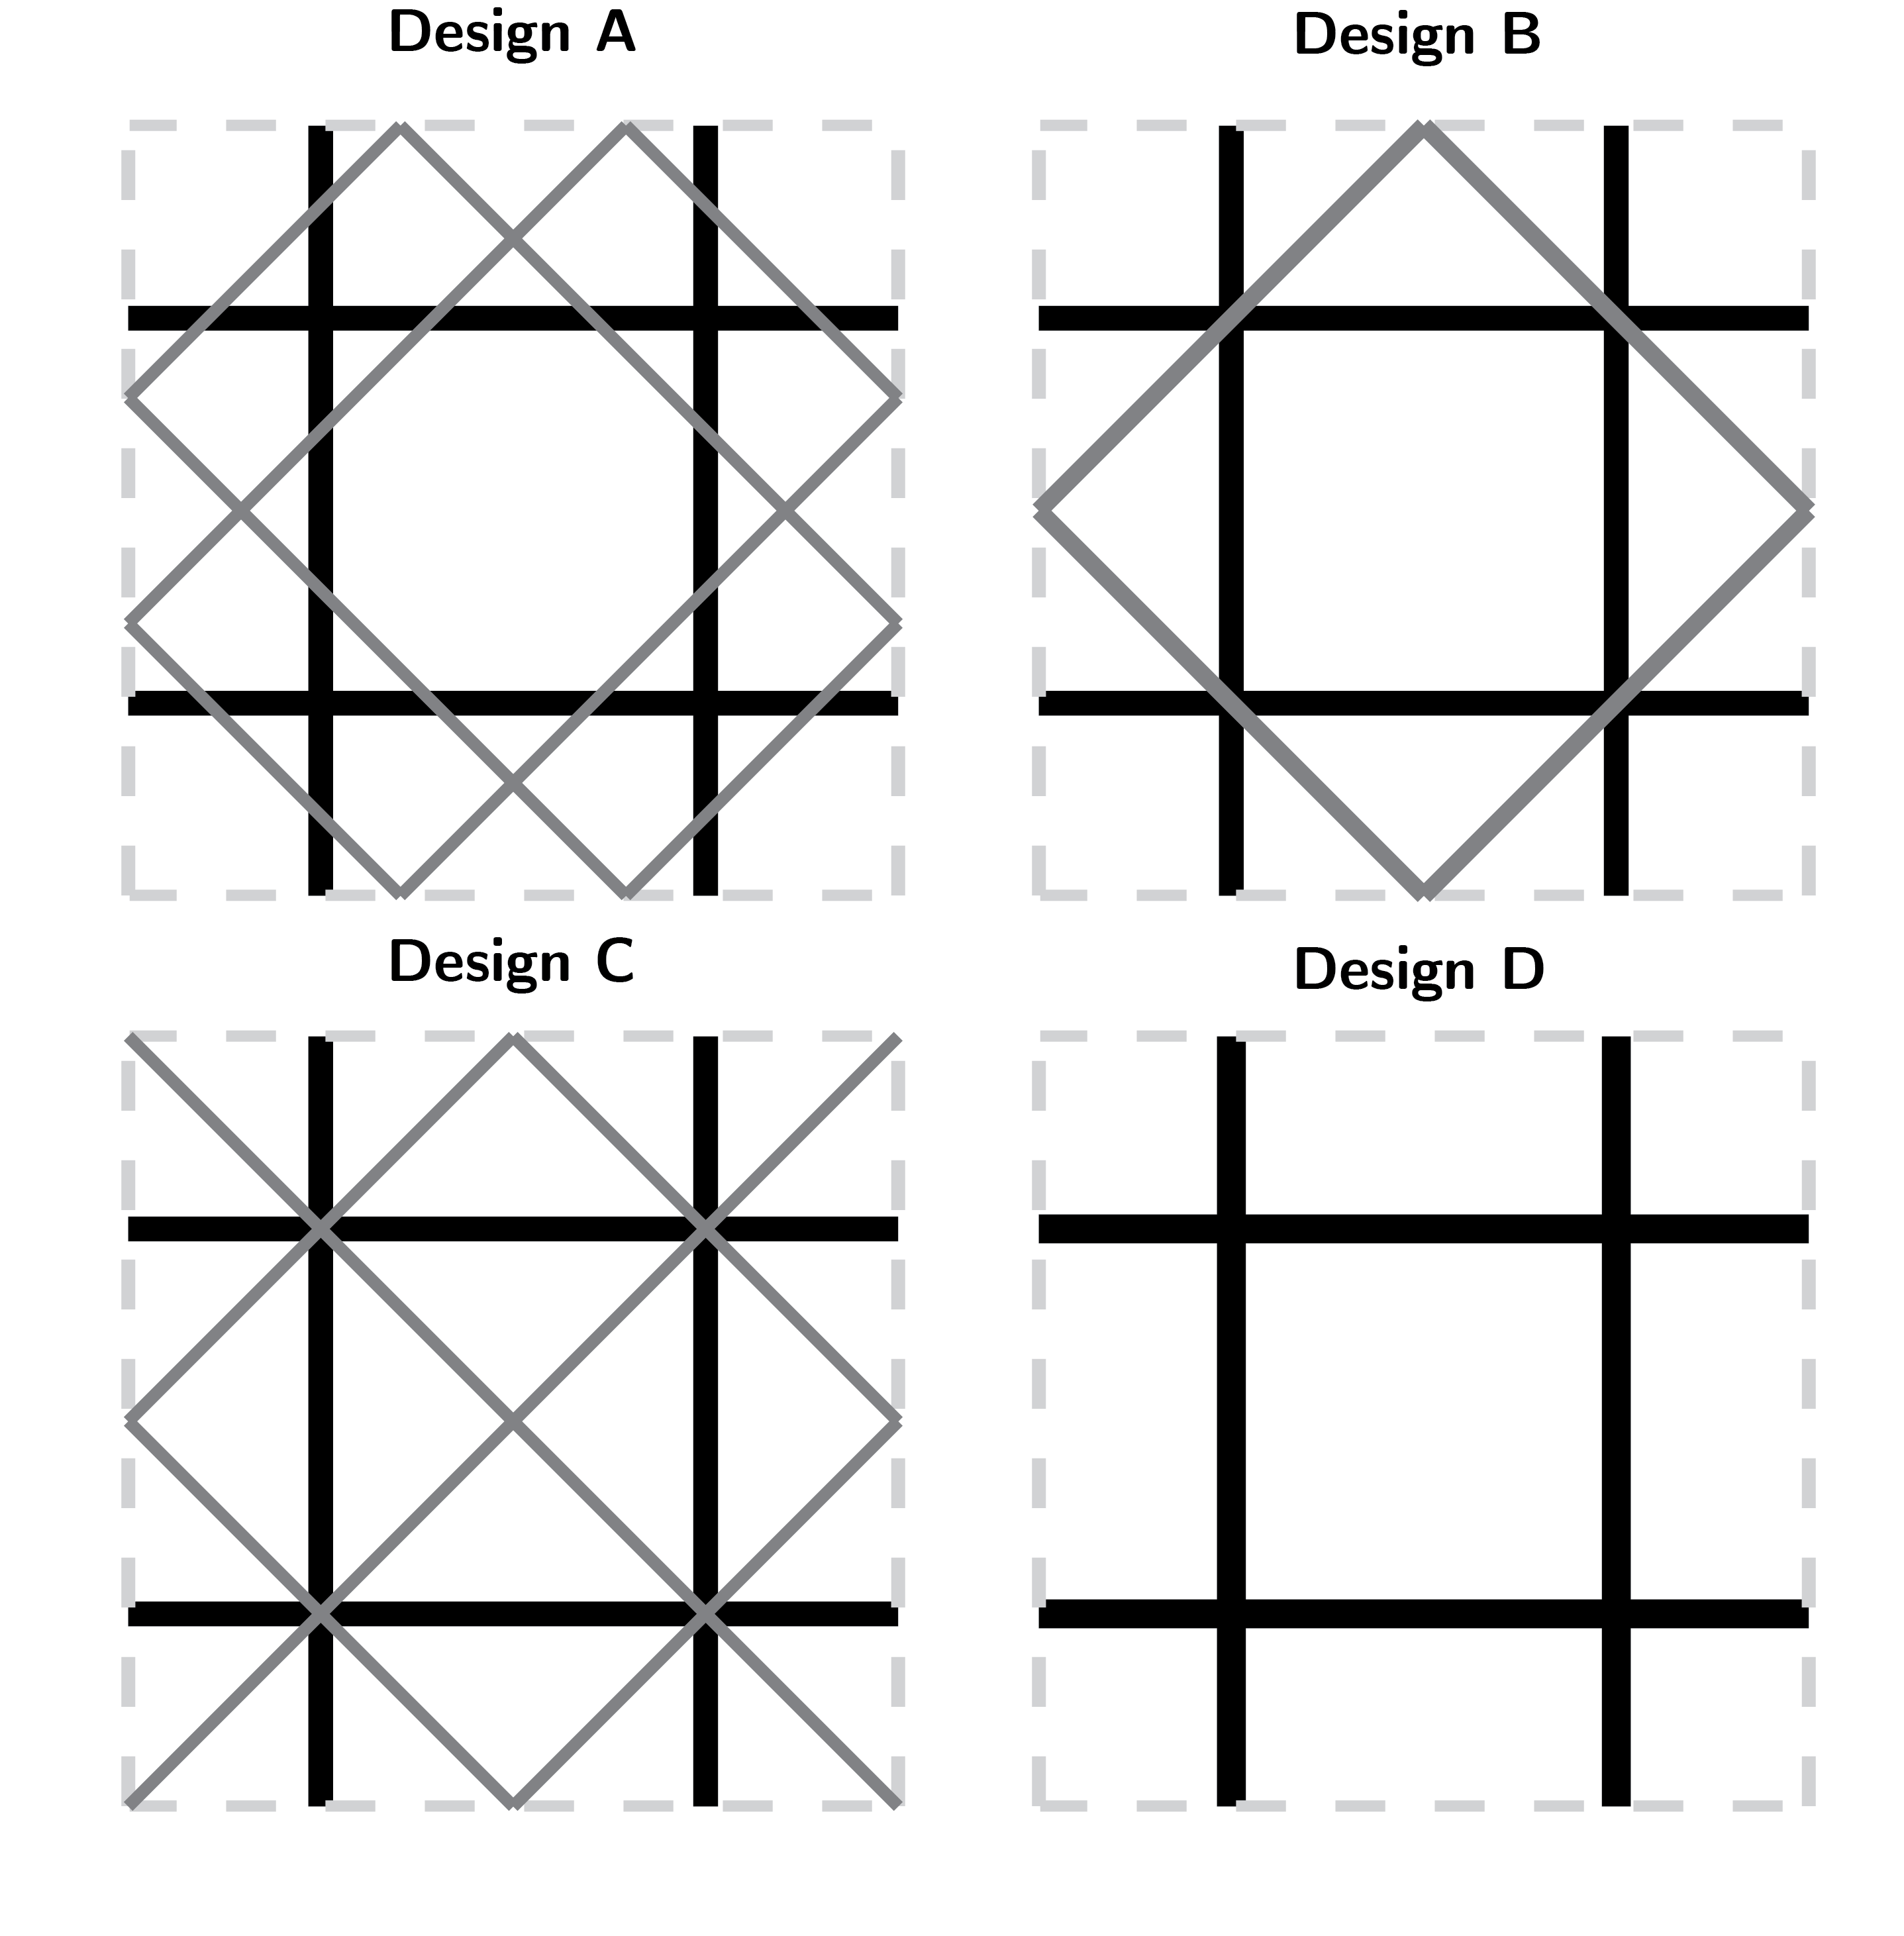
\includegraphics[width=0.6\linewidth]{SFig10.png}
	\caption{{\bf RVE used for the different designs.} This figure portrays the different RVEs used for the different designs considered. Each unit cell is shifted by half of a square cell to the horizontally and half of a square cell  vertically. Periodic boundary conditions are applied on the nodes that intersect with the light gray dashed line.}
	\label{RVE}
\end{figure}

\section{Optimization Analysis}
In an effort to identify lattice configurations resulting in large critical loads, we used  a Python
implementation of the Covariance Matrix Adaptation Evolution
Strategy (CMA-ES) \citep{hansen2003}.  CMA-ES is an evolutionary
algorithm that is used to solve optimization/inverse problems
by iteratively solving several forward problems to adjust
a covariance matrix of the solution. CMA-ES is a derivative
free algorithm, well suited for optimization problems of
high dimensionality. 


\KB{this is not very clear. are we optimizing structures with circular or rectangular cross section? Which parameters do we keep fixed? Add a schematic}

\begin{figure}
	\centering
	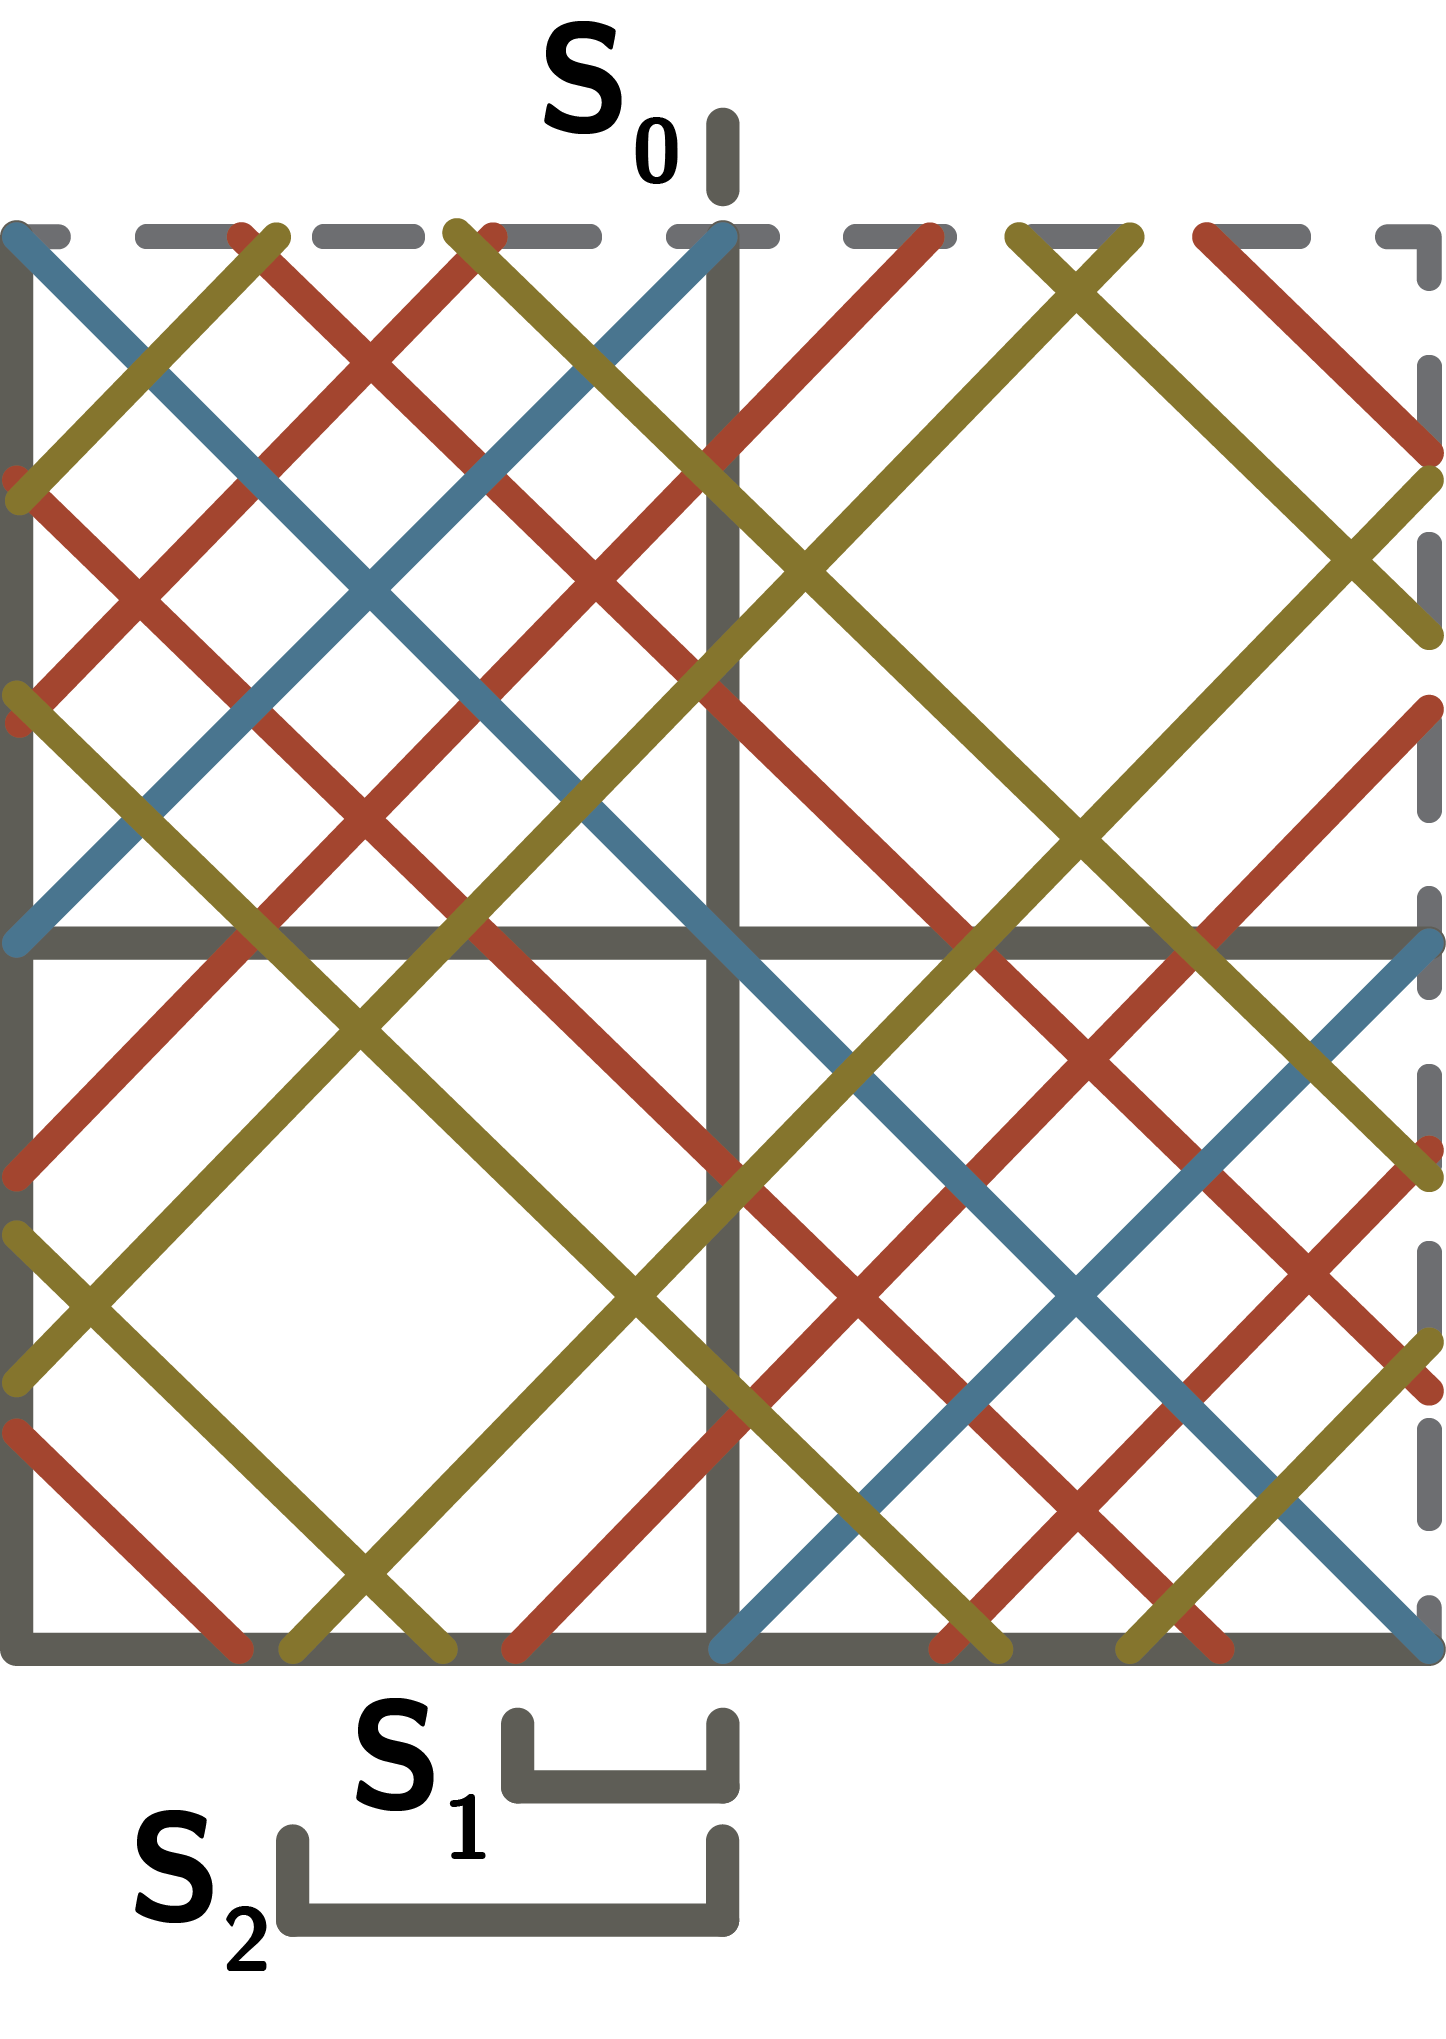
\includegraphics[width=0.25\linewidth]{SFig11.png}
	\caption{{\bf Schematic depicting parameters of Optimization.} This schematic shows an example optimization geometry  at a complexity level of five diagonals. For each set of even diagonals, we allow each diagonal to travel away from each other from the center junction with distances $S_1,S_2$. Note that for every odd diagonal, the distance $S_0=0$ and it is not allowed to vary in order to ensure symmetry.}
	\label{OptimizationSchematic}
\end{figure}

The parameters that need to be determined to achieve large critical loads are: the number of diagonals, the mass ratio ($\lambda$) of non-diagonals to diagonal, and the separation between each even set of diagonals. For this optimization problem, the number of optimization variables increases with the number of diagonal incorporated in the model. Thus, the total number of parameters are $1+(N-1) + (N \text{ mod } 2)/N$ for a given optimization instance with $N$ number of diagonals. An illustration for an optimization structure with $N=5$ is shown \cref{OptimizationSchematic}.

\begin{itemize}
\item the structure's mass ratio $\lambda$ (keeping the total structure volume constant, as well as distributing the mass evenly through all diagonal and non-diagonal elements respectively) and \item the separation of the even numbered diagonal elements from the non-diagonal junction. Separate instances of the optimization algorithm are analyzed for different numbers of diagonal reinforcements. For simulations with odd number of diagonal reinforcements, only an even number of diagonals are separated while keeping one diagonal going through the non-diagonal junction in order to ensure geometry symmetry. 
\end{itemize}

The algorithm's initial values are chosen to be in the center of the design space, namely, $\lambda=1$ and diagonal separation$=0.5*L$. The covariance matrix is initialized uniformly with standard deviation ($\sigma$) half of the domain space, which are normalized to remain between 0 and 1. The optimization is run for uniaxial loading condition in the direction parallel to the non-diagonal elements. 

For the optimization results presented in the main article, we seek to maximize the critical buckling load using a single objective target function. However, an equivalent analysis is performed to maximize the critical buckling strain as the target response (\cref{BucklingOptimization}.) 

\KB{add expression for the target function} 
\\\mf{The target function is simply 1/ buckling reaction force, should we just keep this verbally instead of mathematically?}

\begin{figure}[H]
    \centering
    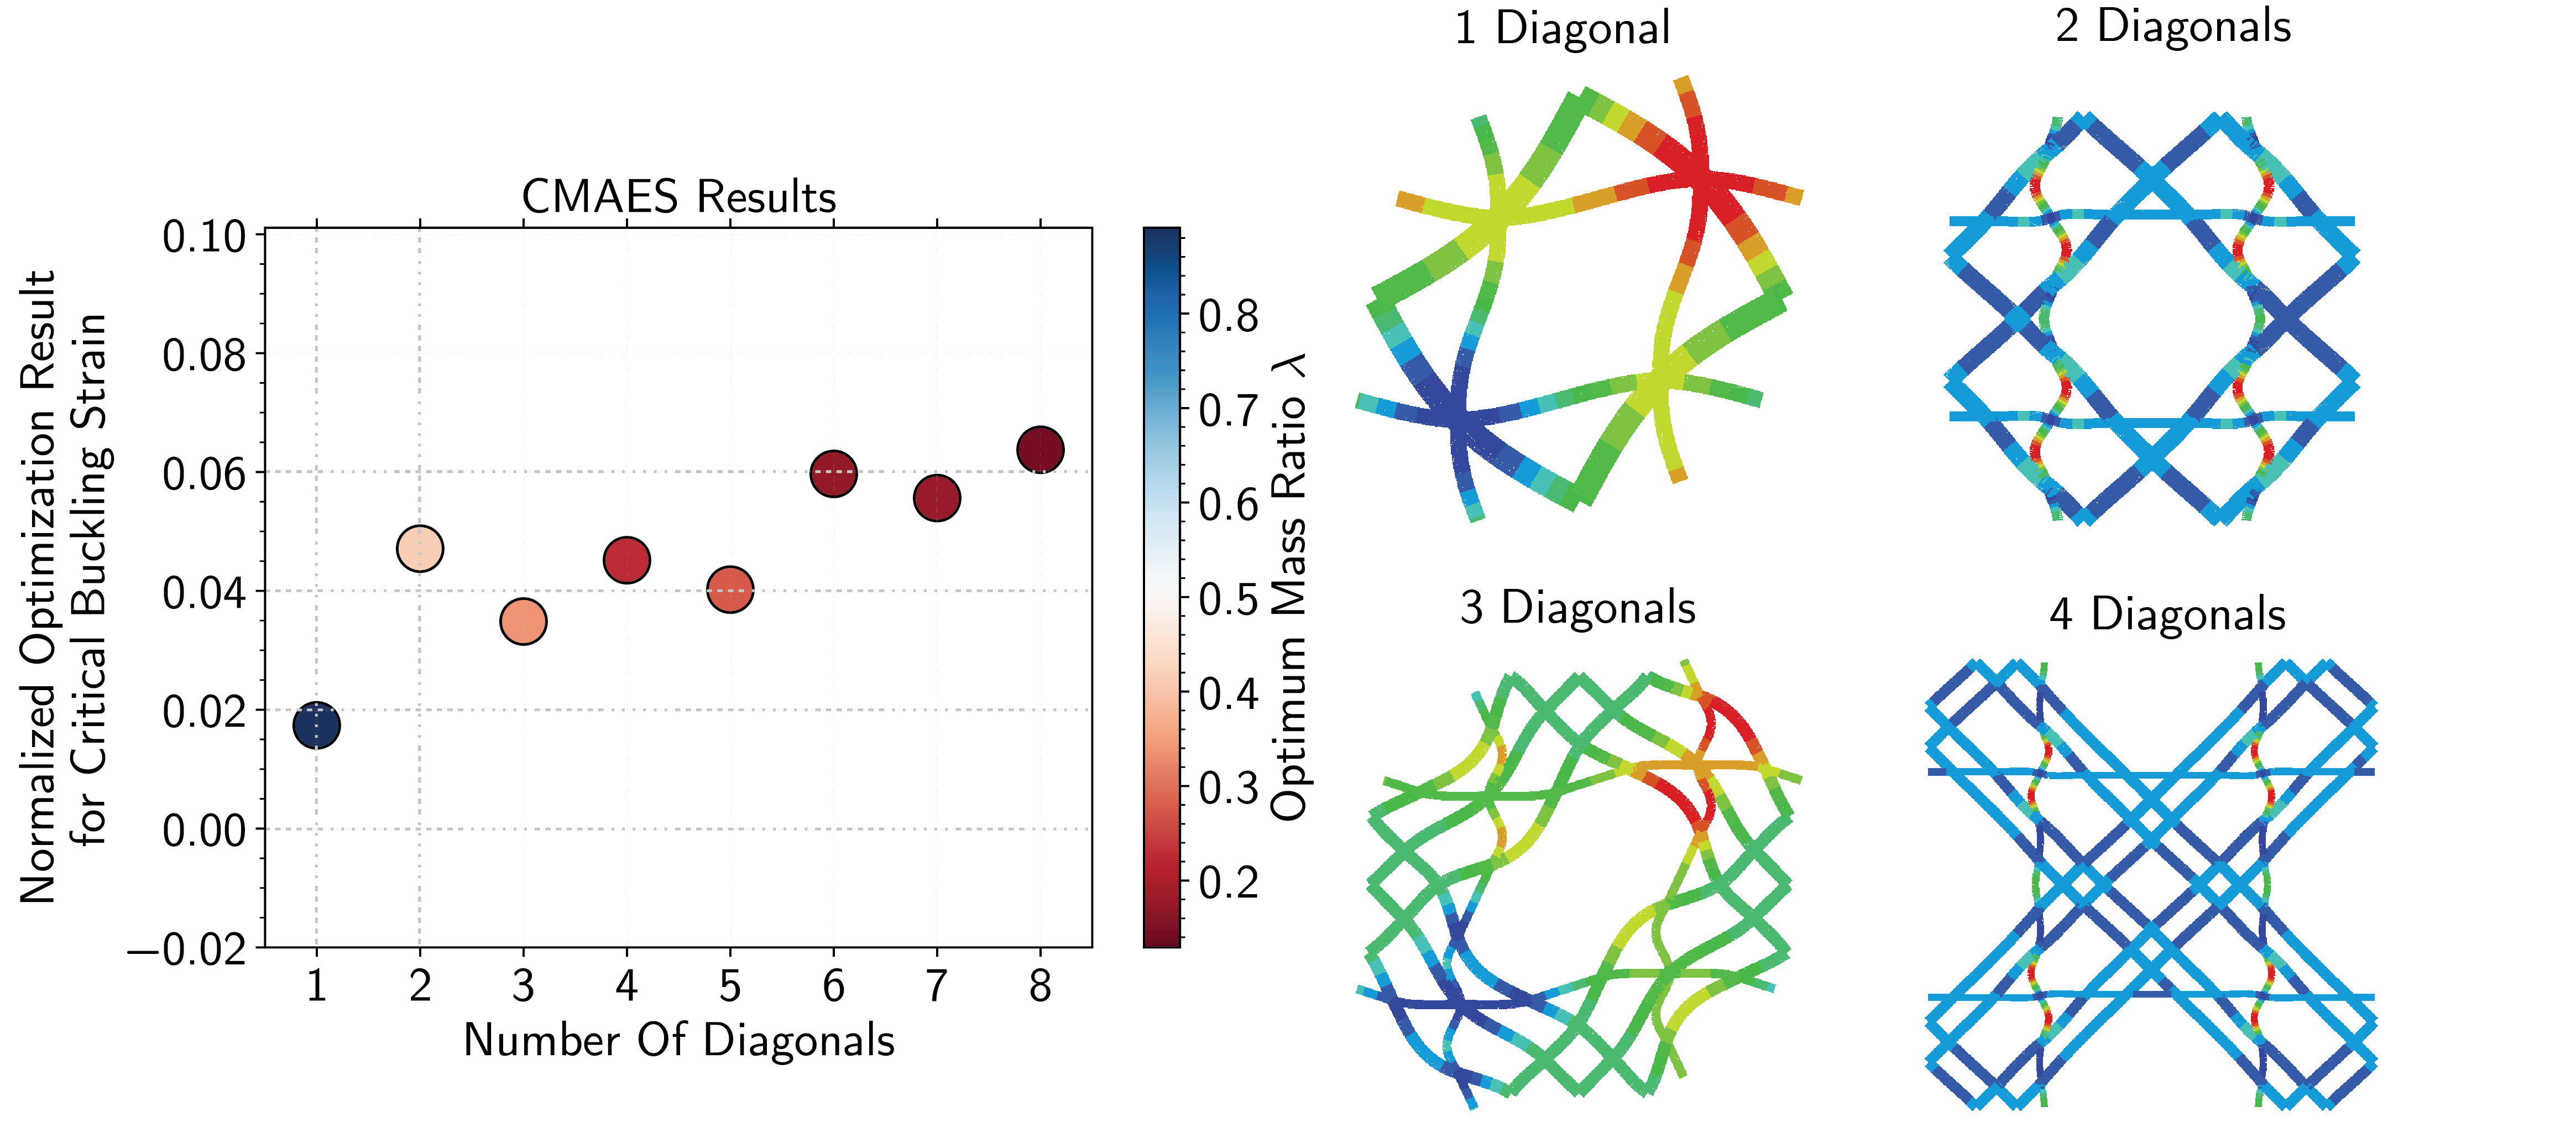
\includegraphics[width=0.9\linewidth]{SFig6.png}
    \caption{{\bf Buckling Optimization.} Graph shows optimal value of critical buckling strain for varying number of diagonals. For all simulations, the total mass of the structure is maintained constant while the mass-ratio is allowed to vary. Furthermore, the diagonal separation for each pair of diagonal is allowed to vary together ensuring half symmetry of the structure at all times. The optimization is run under a uniaxial loading condition. The color of each point on the graph corresponds to the optimum value of mass ratio for that particular number of diagonals. Four deformation plots of the optimum structure and buckling modes are provided on the right for their respective number of diagonals.}
    \label{BucklingOptimization}
\end{figure}

\section{Circular Cross-Section Results}
The results presented here complement that found on the main article and show that the structural benefit for the Design A persists when using a different cross-section for the structure. We show that for varying loading angles all of the diagonally reinforced designs provide the same stiffness, but Design A consistently provides the best resistance to buckling. 

\begin{figure}[H]
	\centering
	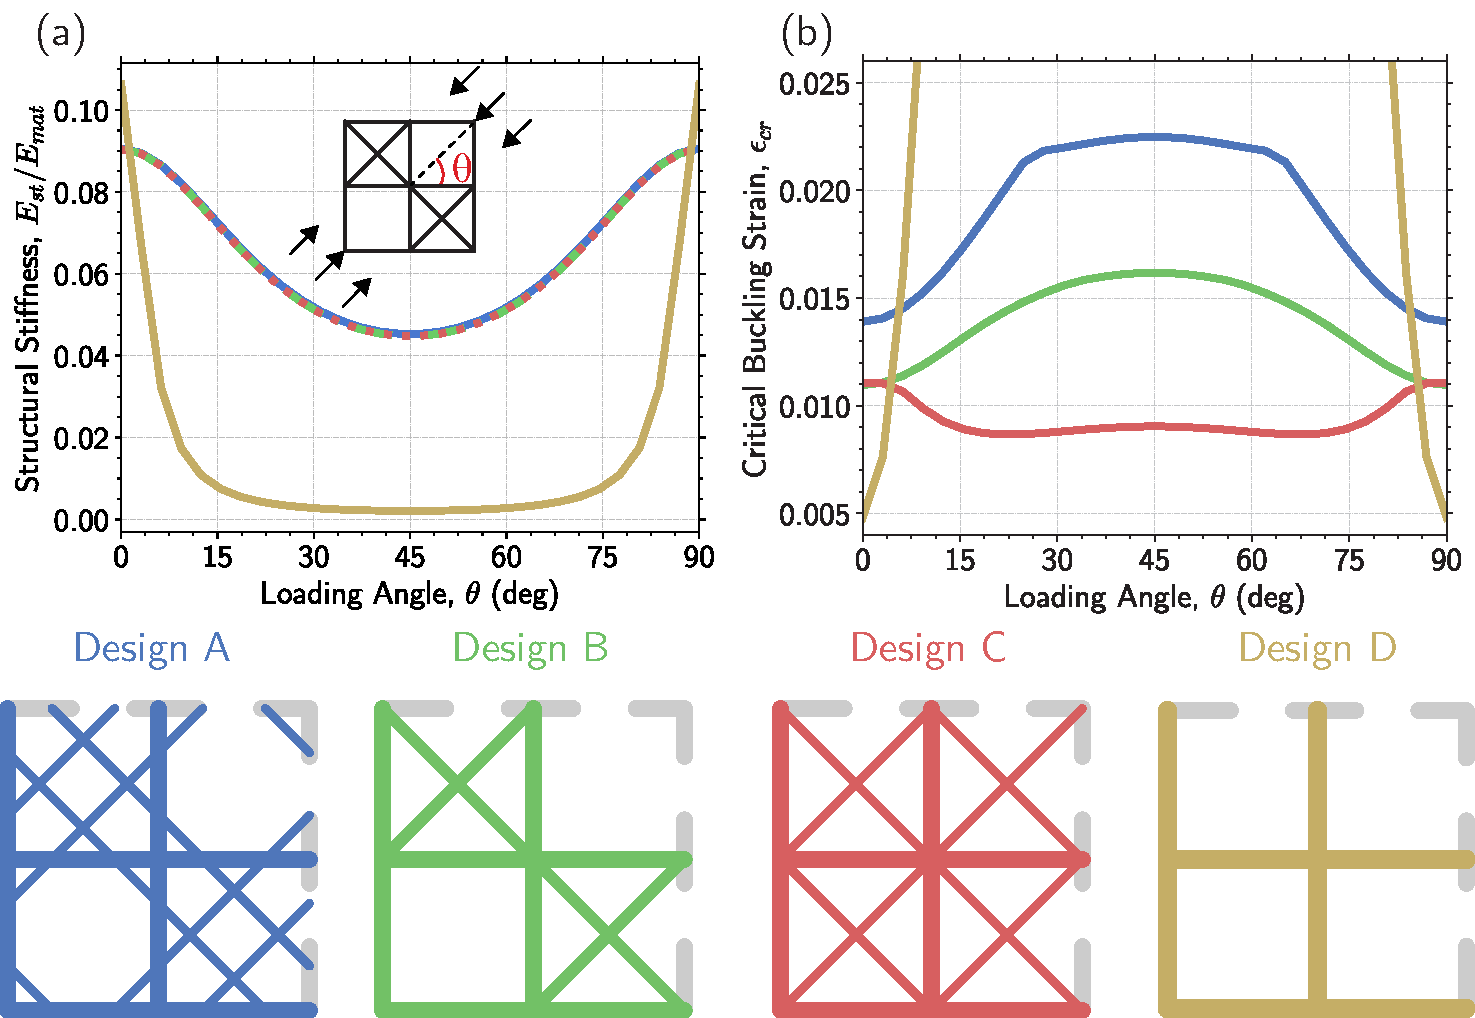
\includegraphics[width=0.6\linewidth]{SFig7.pdf}
	\caption{{\bf Circular Cross Section Results.} The color of the lines correspond to it's respective design color below the plots. (a) Shows the linear elastic stiffness of the different designs as a function of the loading angle. All structures except for the design without diagonal reinforcement have the same stiffness. (b) Shows the critical buckling strain for varying loading angle. For all angles, Design A outperforms other diagonally reinforced designs. These results show that the two diagonal benefit persists beyond a particular beam cross-section design.}
	
	\label{CircularCrossSection}
\end{figure}
\section{Parameter Exploration}
In order to survey the design space of the double diagonal construction we explore parametric simulations for 2 variables: diagonal separation and mass ratio. For each of these separate analysis, we maintain the sponge geometry as our base geometry and vary only the respective variable. 

\subsection{Rectangular Cross Section}\label{sec:rectparam}
This section shows the results when using a rectangular cross-section for the truss members. From \cref{SquareCrossSectionParameter}(a) it is apparent that there exists an optimum for the diagonal separation that occurs when the spacing between diagonals are approx 0.2 of the horizontal distance between vertical struts. This optimum value also persists when varying the loading angle. From \cref{SquareCrossSectionParameter}(b) it can be seen that the linear stiffness is symmetrically and almost purely dependent on the mass ratio allocated to diagonal versus non-diagonal elements. Comparing this figure to \cref{CircularCrossSectionParameter}(b) we can also see that even the design cross-section does not change the linear stiffness behavior.  \cref{SquareCrossSectionParameter}(c) shows that there exists two optimum mass ratios, one where more material is allocated to the diagonal and one where there is more material allocated to non-diagonals.  Note that if more matterialk

\begin{figure}[H]
	\centering
	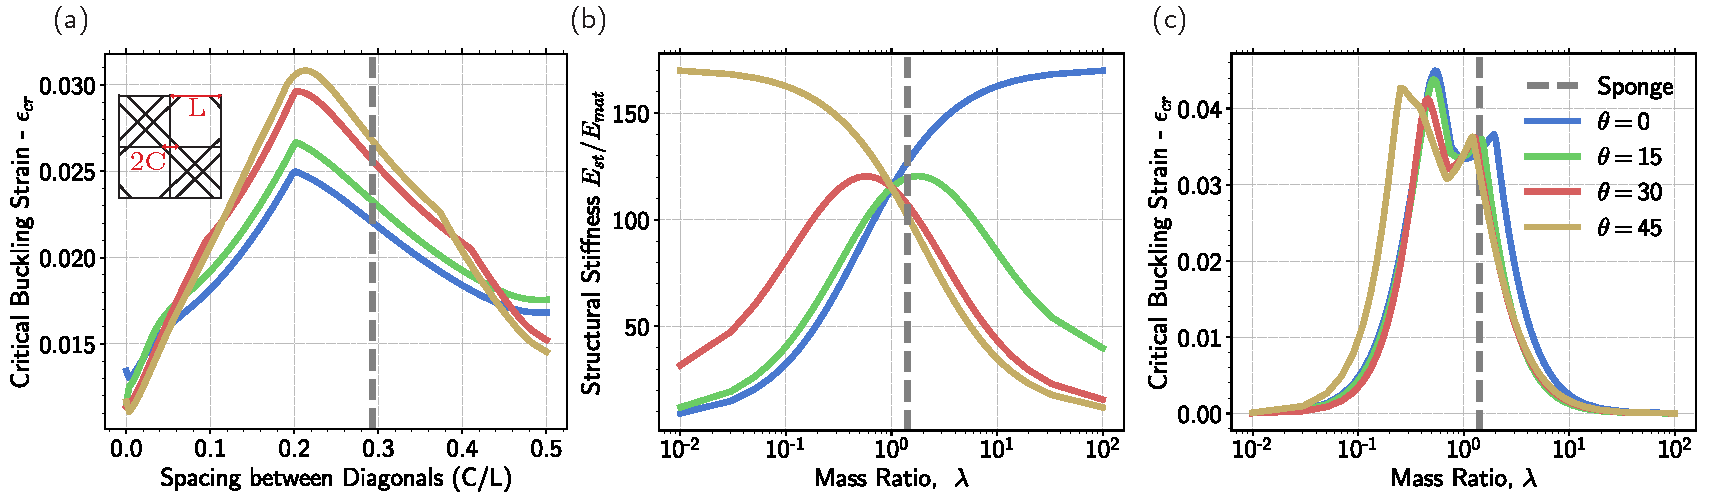
\includegraphics[width=0.9\linewidth]{SFig8.pdf}
	\caption{{\bf Rectangular Cross Section Parameter Exploration.} For each of these plots, we vary a single parameter while maintaining the base sponge inspired geometry constant. The gray line indicates the sponge design parameter. (a) Shows the critical buckling strain for varying spacing between diagonals. (b) Shows the structural stiffness of the geometry as we vary the mass ratio $\lambda$. (c) Shows the critical buckling strain of the geometry as we vary the mass ratio $\lambda$.}
	\label{SquareCrossSectionParameter}
\end{figure}

\subsection{Circular Cross Section}
For this cross-section we stay consistent with the natural sponge, and we can see from \cref{CircularCrossSectionParameter} the overall behavior has second order differences for (a), no change for (b) and a large difference in relative magnitude for (c).  Furthermore, we can see from the comparison between this section and \cref{sec:rectparam} that by using a rectangular cross-section we can tune the mass ratio to achieve an overall structure with higher critical buckling strength. 

\begin{figure}[H]
	\centering
	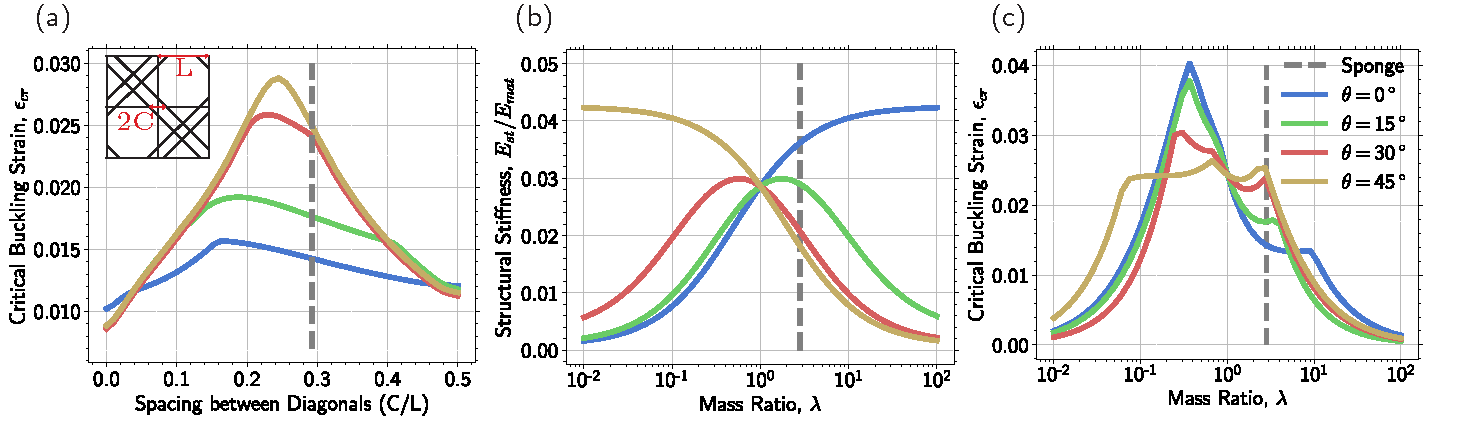
\includegraphics[width=0.9\linewidth]{SFig9.pdf}
	\caption{{\bf Circular Cross Section Parameter Exploration.} For each of these plots, we vary a single parameter while maintaining the base sponge inspired geometry constant. The gray line indicates the sponge design parameter. (a) Shows the critical buckling strain for varying spacing between diagonals. (b) Shows the structural stiffness of the geometry as we vary the mass ratio $\lambda$. (c) Shows the critical buckling strain of the geometry as we vary the mass ratio $\lambda$.}
	\label{CircularCrossSectionParameter}
\end{figure}

\section{Local and Global Instabilities}
\mf{How should I go about describing this here?}

% Bibliography
%\nocite{aizenberg2005}
%\nocite{deshpande2001}
%\nocite{miserez2008}
%\nocite{weaver2010}

\bibliography{refs}
\bibliographystyle{apalike}
% \bibliographystyle{plainnat}

\end{document}